\documentclass[12pt, a4paper]{article}

\usepackage[utf8]{inputenc}
\usepackage[hmargin=2.5cm,vmargin=2.5cm]{geometry}
\usepackage[brazil]{babel}
\usepackage{graphicx}
\usepackage{amsmath}
\usepackage{steinmetz}
\usepackage{float}
\usepackage{graphicx}


\begin{document}

{\large
\centerline{\textbf{Tarefa 12 - OmpCloud}}
\centerline{\textbf{Introdução à Programação Paralela}}
\centerline{\textbf{Gustavo Ciotto Pinton 117136}}
}

\section{Exercício}

A tabela \ref{tab:resultados}, logo abaixo, contém dados de execuções variando
\(N\) de 100 até 5000 para um \textit{cluster Spark} com 6 nós (2
\textit{masters} e 4 \textit{workers}) criado no leste do Canadá, conforme
figura \ref{fig:dashboard}. Todos os testes foram executados no
\textit{parsusy} e os tempos das execuções \textit{serial} e paralelo estão
representados em segundos. Adicionalmente, foram utilizadas as \textit{flags} \texttt{--executor-memory 15g}, \texttt{--driver-memory 15g},
\texttt{--driver-cores 8} e \texttt{--executor-cores 8} para a configuração
do ambiente de execução nos nós da \textit{cloud}.

\begin{table}[h]
    \centering
	\caption{\label{tab:resultados} Resultados obtidos para alguns valores de \(N\).} 
	\begin{tabular}{| c | c | c | c | c | c | c | c |}
		\hline
		 & \textbf{100} & \textbf{1000} & \textbf{1500} & \textbf{2000} &  \textbf{2500} & \textbf{3500} & \textbf{5000}\\\hline 
		 Serial (s) & 0.015  & 8.294 & 31.459 & 87.655 & 251.407 & 861.234 & 2505.961 \\\hline 
		 Paralelo (s) & 63.035 & 79.315 & 75.004 & 87.323 & 107.012 & 175.825 & 349.596 \\\hline 
		 Speedup & 0.0002 & 0.105  & 0.419  & 1.004 & 2.349 & 4.898 & 7.168 \\\hline
		
	\end{tabular}
\end{table}

\begin{figure}[h!] 
    \centering
    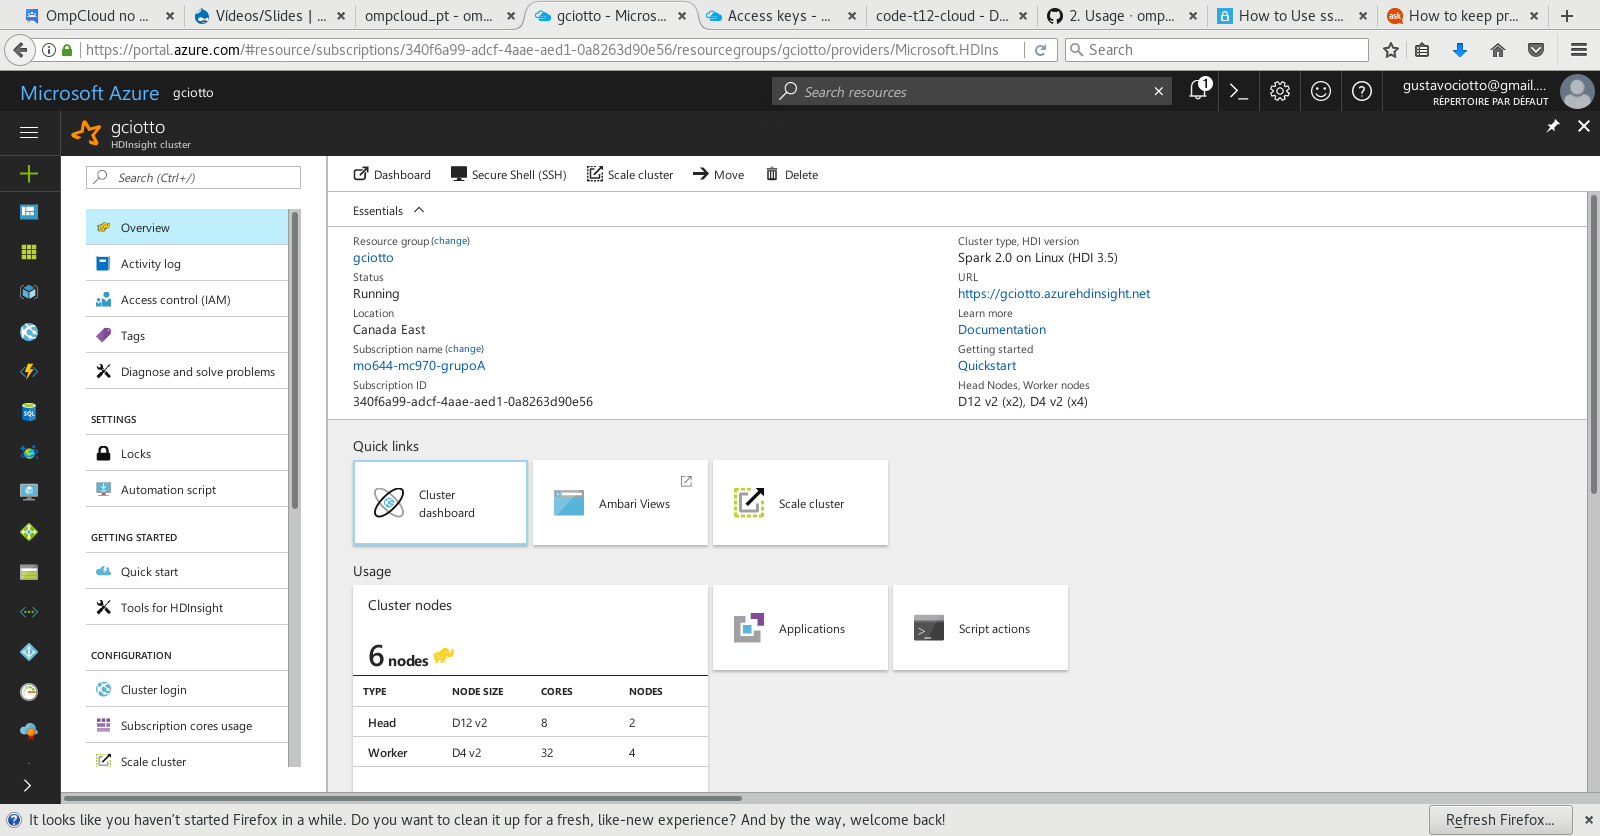
\includegraphics[width=\textwidth]{img/dashboard}
    \caption{Sumário do \textit{cluster} criado.}        
    \label{fig:dashboard}
\end{figure}


Verifica-se, portanto, que os custos de \textit{offloading} (\textit{download}
e \textit{upload} de dados para/da \textit{cloud}) não justificam o uso do
\textit{OmpCloud} para valores de \(N\) inferiores a 2000. Evidentemente, tal
valor depende também da qualidade da conexão internet e da localidade das máquinas
criadas no \textit{Azure}.

\vspace{12pt}

As figuras \ref{fig:nodes} e \ref{fig:event} são capturas de tela da
interface \textit{web} de monitoração do \textit{Spark} para a execução com \(N=100\). É possível
observar, através da primeira, quais nós foram utilizados para o processamento
e qual deles foi usado como \textit{master} e, a partir da segunda, a fração de
tempo em que cada fase correspondente à primeira claúsula \texttt{data map}
levou para ser executada.

\begin{figure}[h!] 
    \centering
    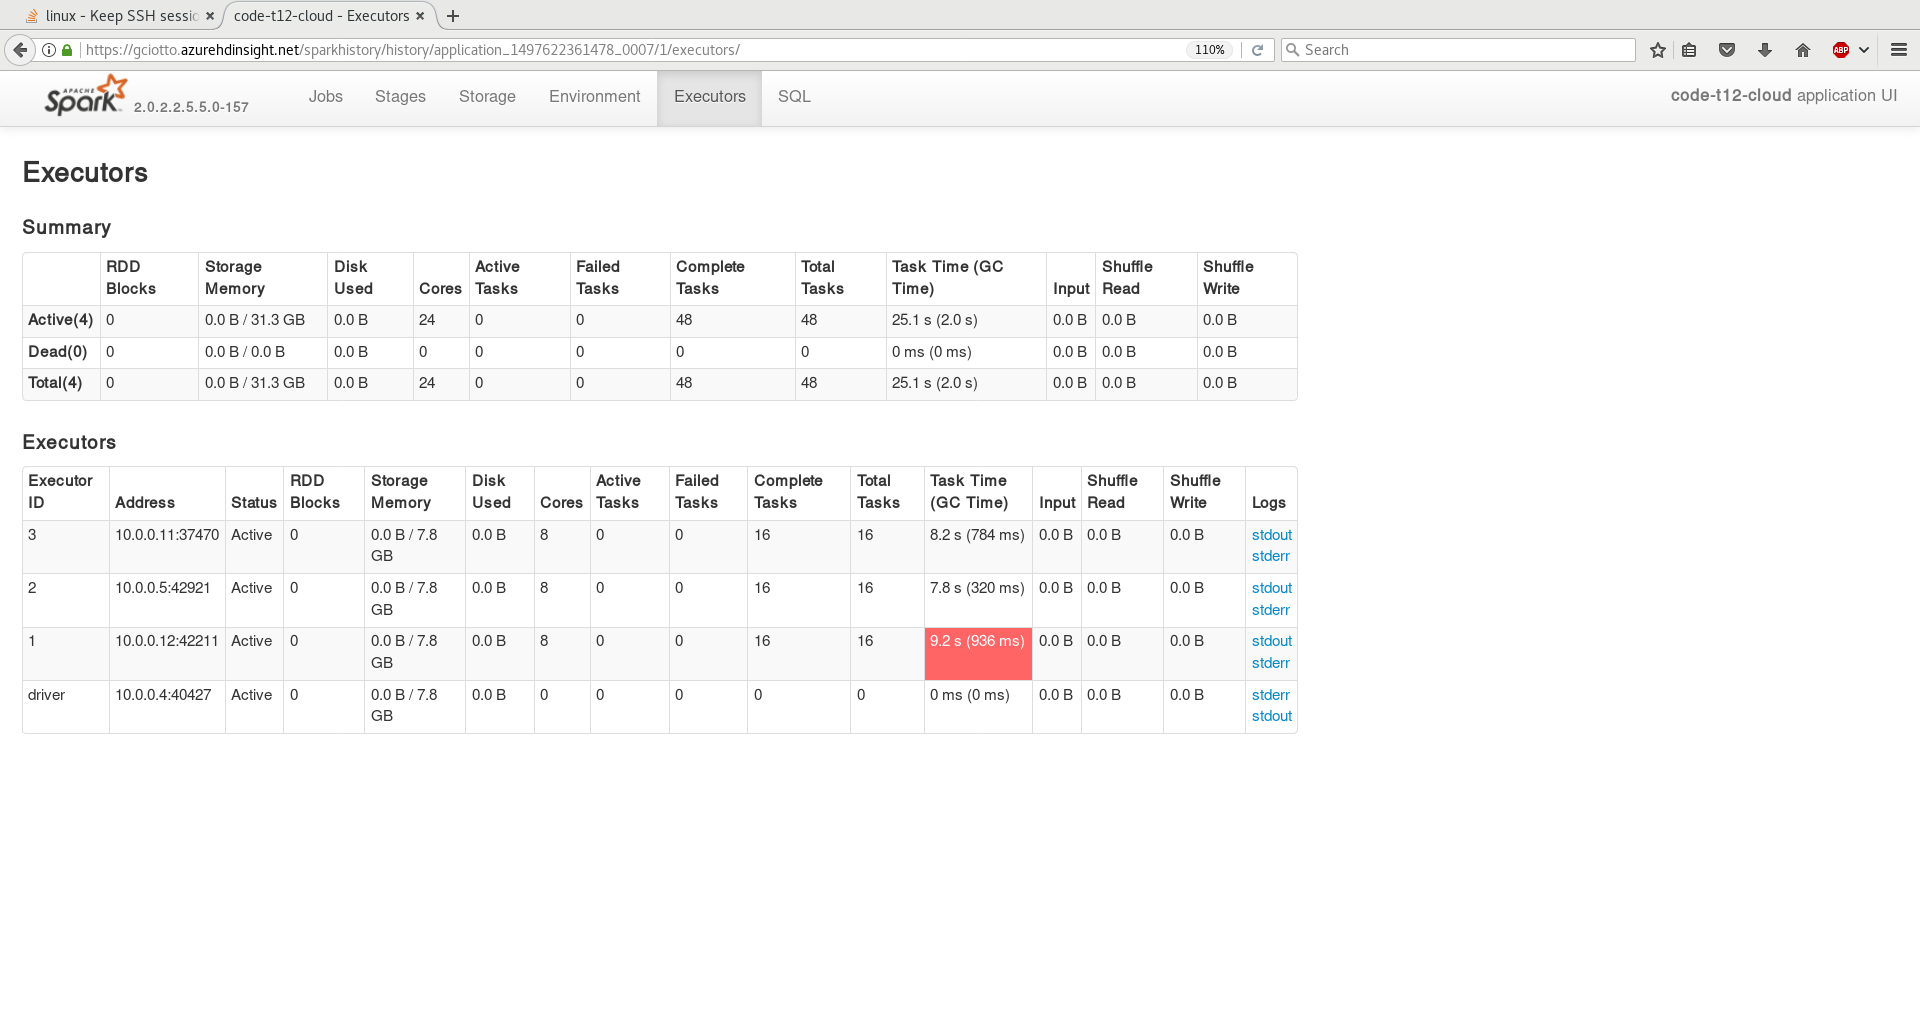
\includegraphics[width=\textwidth]{img/100/executors}
    \caption{Divisão das tarefas entre os nós do \textit{cluster}.}        
    \label{fig:nodes}
\end{figure}

\begin{figure}[h!] 
    \centering
    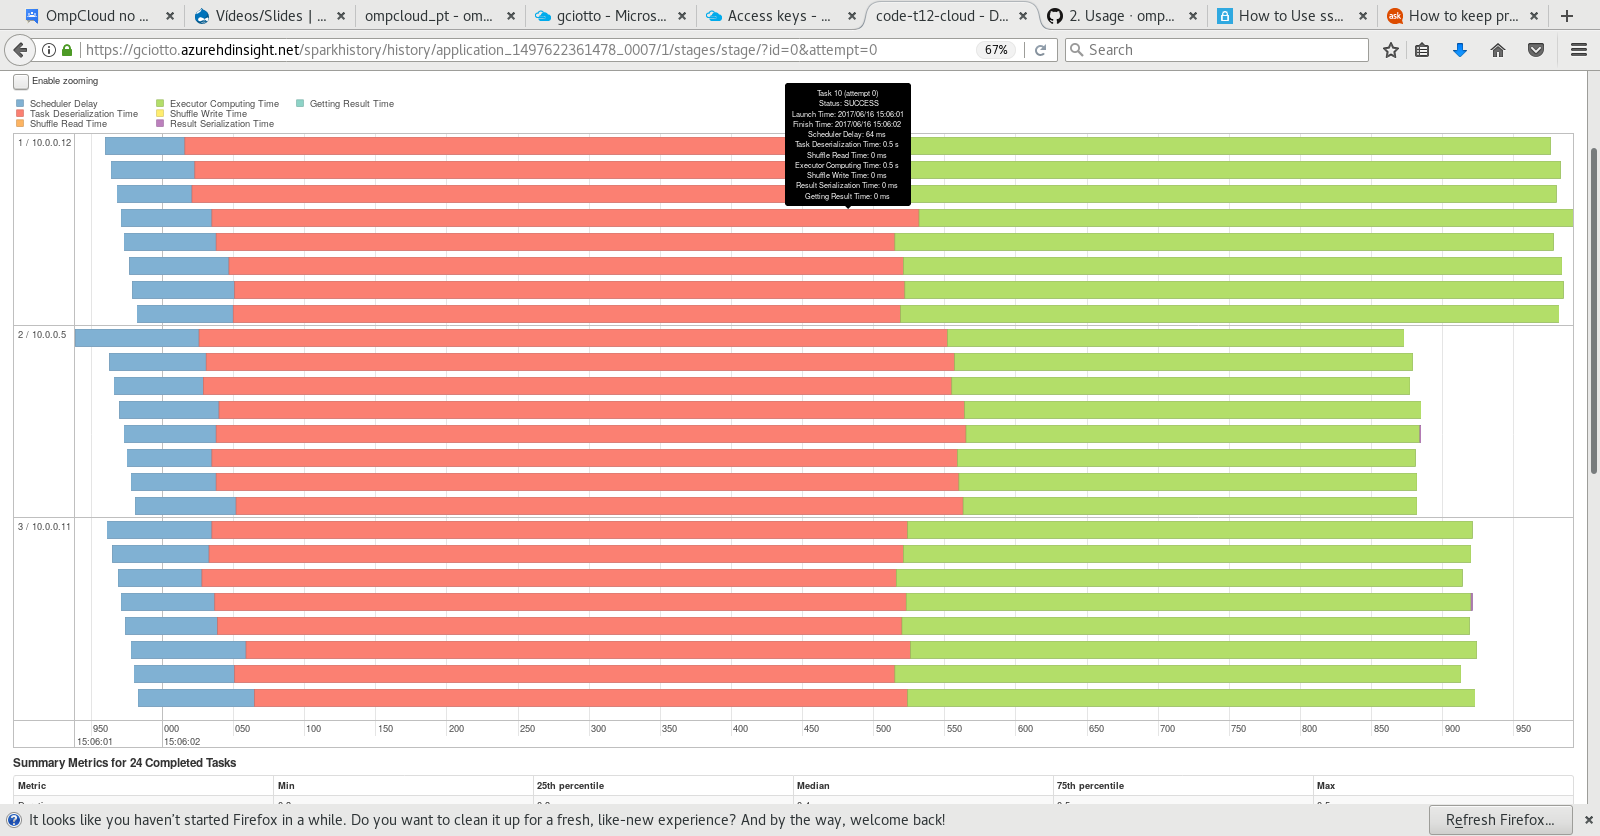
\includegraphics[width=\textwidth]{img/100/event}
    \caption{Fração de tempo consumida pelas tarefas da primeira claúsula
    \texttt{data map} entre os nós do \textit{cluster} para \(N = 100\).}
    \label{fig:event}
\end{figure}

Observa-se a presença de quatro nós neste caso. Três deles agem como
\textit{executor}, enquanto que o quarto, como \textit{driver} ou
\textit{master}.

\vspace{12pt}

A figura \ref{fig:event5000}, por sua vez, foi obtida para \(N = 7500\).
Verifica-se que, em comparação com a imagem \ref{fig:event}, a fração correspondente ao tempo de
computação (barra verde) para \( N = 7500\) é muito superior ao caso \(N =
100\). Tal fato se traduz em um maior \textit{speedup} para o último caso,
visto que um volume maior de cálculo é transferido da CPU para os
nós da \textit{cloud}. Observa-se também, que o intervalo de
\textit{offloading} é muito inferior àquele de computação, indicando, desta
forma, que todo o \textit{overhead} de transferência de dados pode ser
completamente justificado pelos ganhos produzidos pela computação distribuída.

\begin{figure}[h!] 
    \centering
    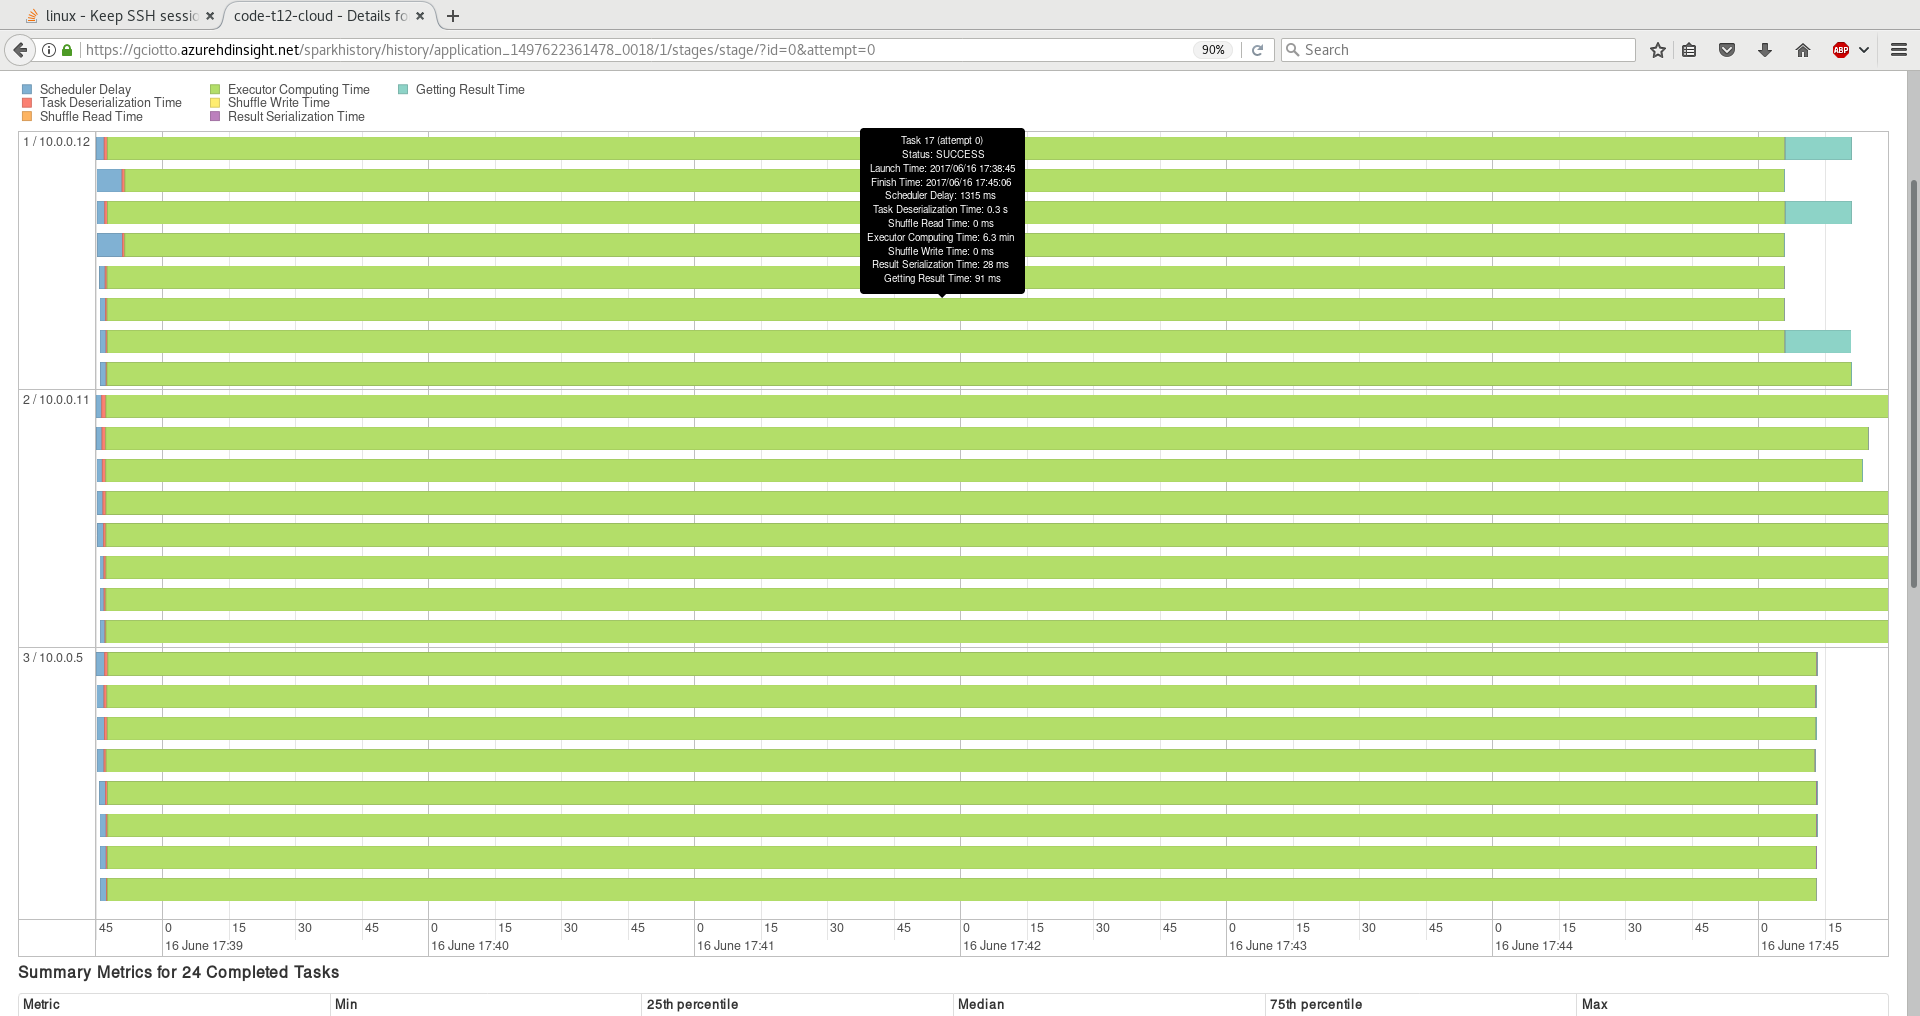
\includegraphics[width=\textwidth]{img/7500/event}
    \caption{Fração de tempo consumida pelas tarefas da primeira claúsula
    \texttt{data map} entre os nós do \textit{cluster} para \(N = 7500\).}        
    \label{fig:event5000}
\end{figure}

\end{document}
